\documentclass{article}
\usepackage[utf8]{inputenc}
\usepackage[T1]{fontenc}
\usepackage{ngerman}
\usepackage{graphics}
\usepackage{pdfpages} 
 
\title{Künstliche Intelligenz\\~\\Hausaufgabe 4\\ \small{N. Lehmann, A. Zubarev}}
\date{21.05.2015}

\begin{document}

\maketitle

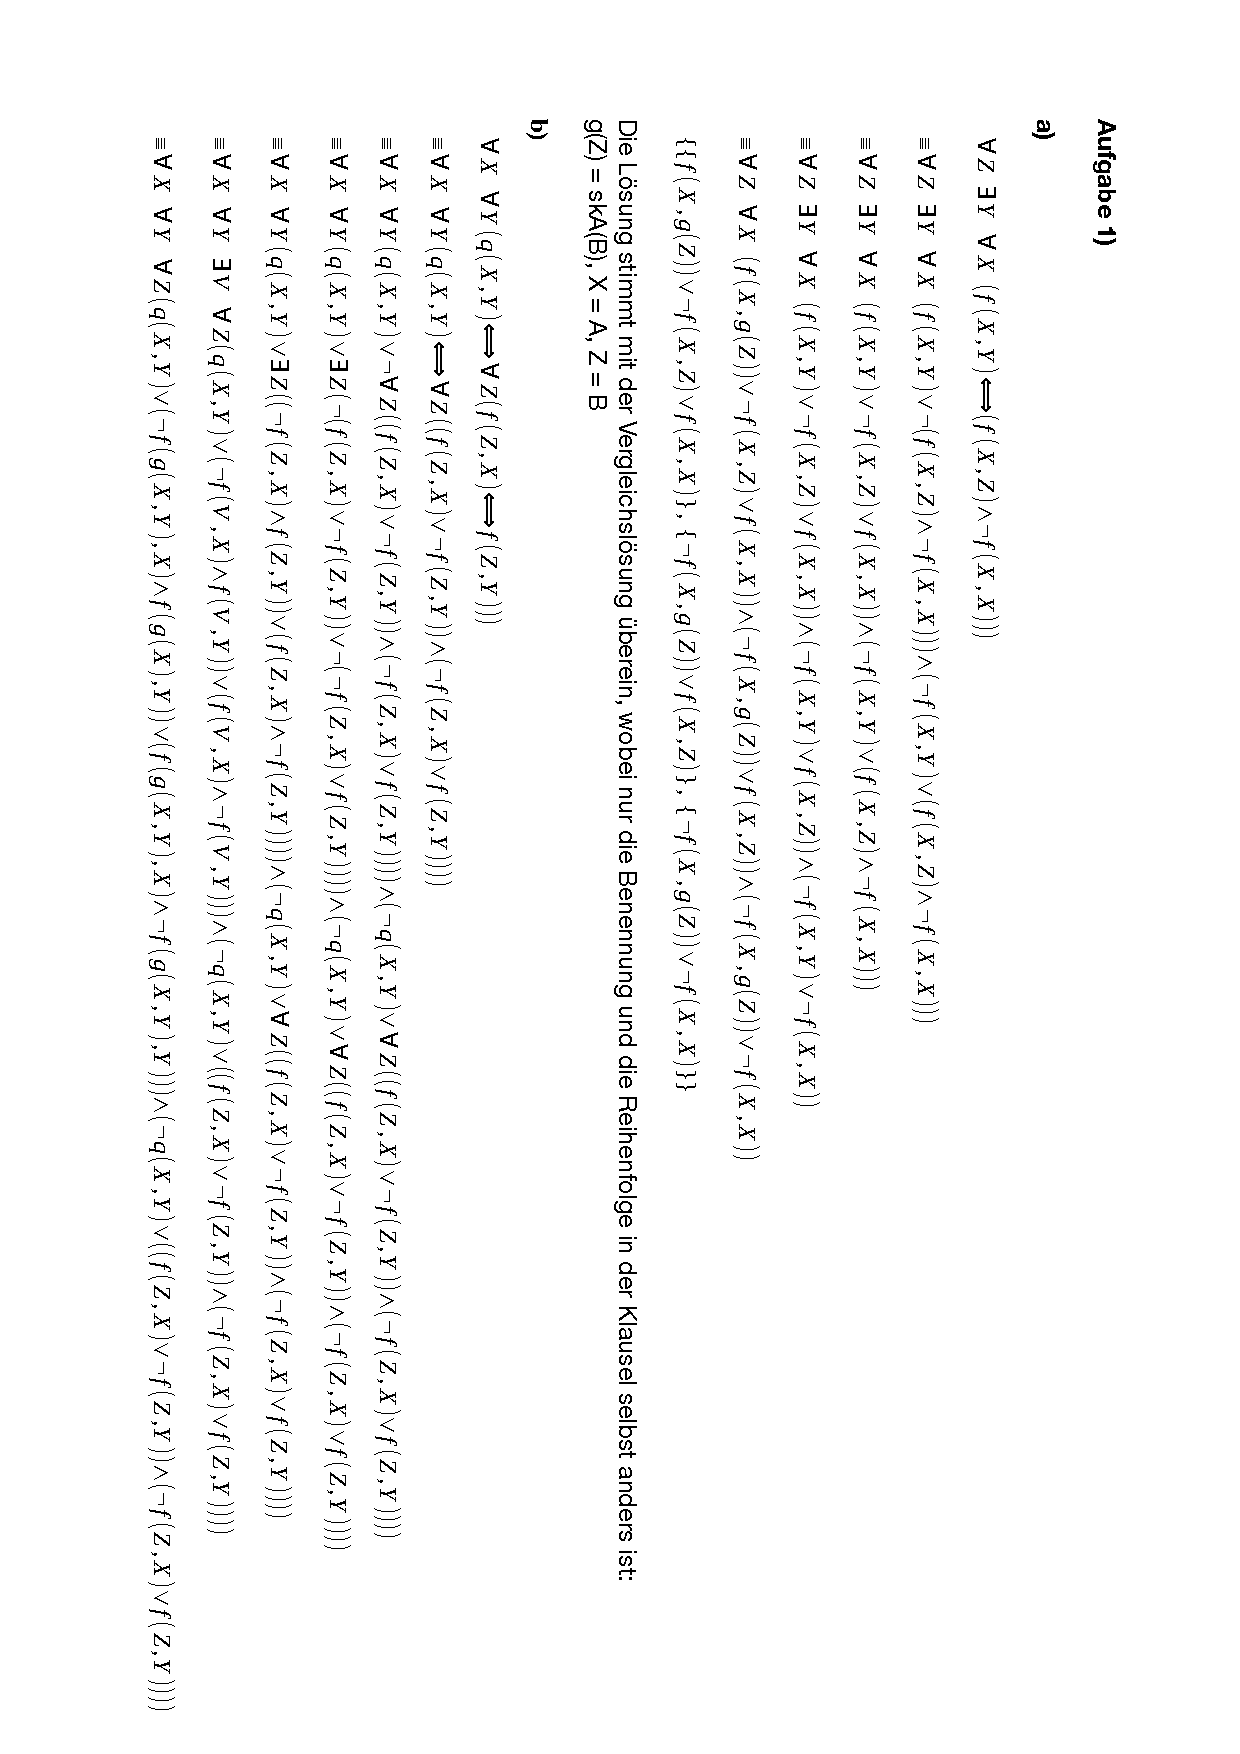
\includepdf[pages=1-4]{ki_hw_04_a01.pdf}

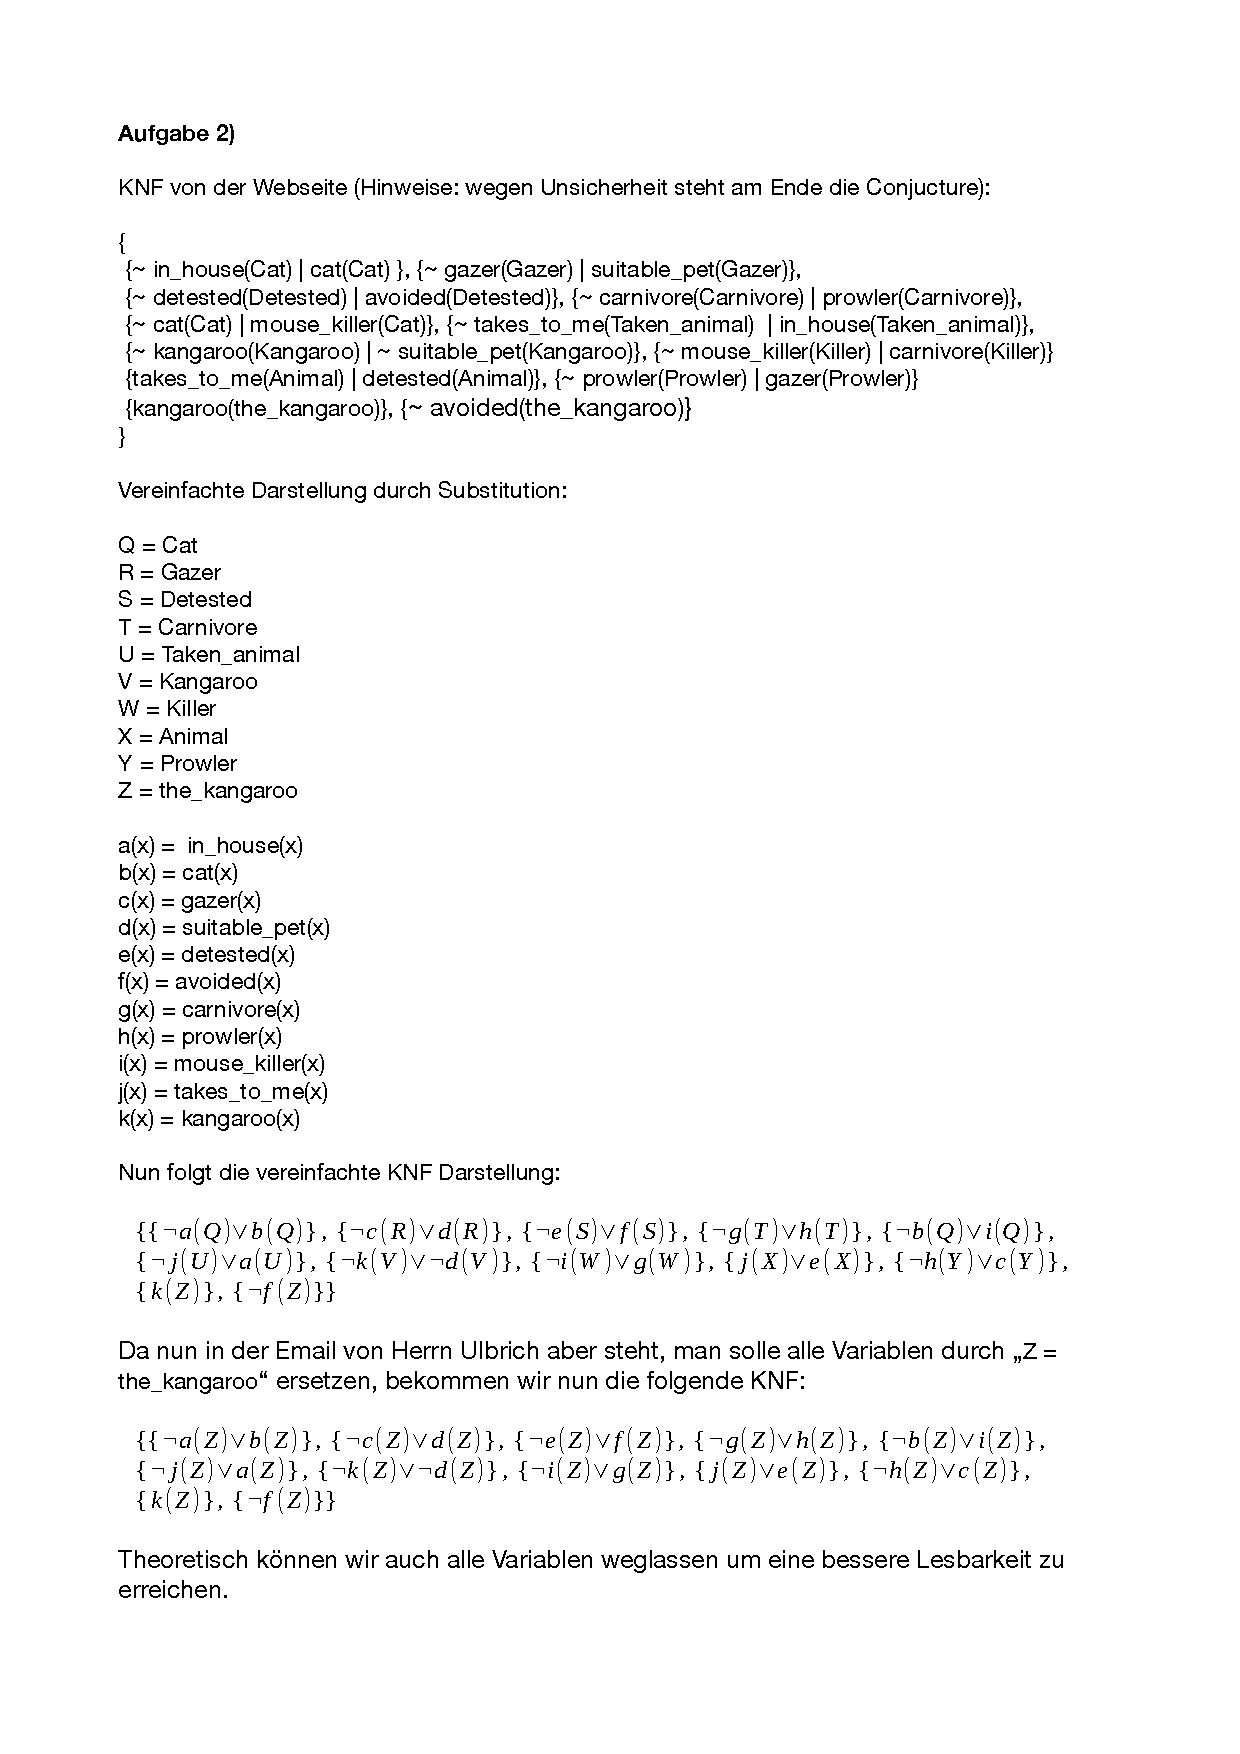
\includepdf[pages=1-6]{Ki_u4_a2.pdf}\newpage

\section*{Aufgabe 3: Herbrand Interpretation}

$V = \{X,Y\}$\\
$F = \{vater\_von/1, mutter\_von/1, max/0\}$\\
$P = \{verheiratet/2 \}$\\
\\
\underline{Herbrand Intepretation}:\\

$H_{Universum}$ = $\{$\\
$max$,\\
$vater\_von(max)$,\\
$mutter\_von(max)$,\\
$vater\_von(vater\_von(max))$,\\
$vater\_von(mutter\_von(max))$,\\
$mutter\_von(vater\_von(max))$,\\
$mutter\_von(mutter\_von(max))$,\\
$vater\_von(vater\_von(vater\_von(max)))$,\\
$vater\_von(mutter\_von(vater\_von(max)))$,\\
$vater\_von(vater\_von(mutter\_von(max)))$,\\
$vater\_von(mutter\_von(mutter\_von(max)))$,\\
$mutter\_von(vater\_von(vater\_von(max)))$,\\
$mutter\_von(mutter\_von(vater\_von(max)))$,\\
$mutter\_von(vater\_von(mutter\_von(max)))$,\\
$mutter\_von(mutter\_von(mutter\_von(max)))$,\\
...\\
$\}$

\newpage

$H_{Basis}$ = $\{$\\
$verheiratet(max,max)$,\\
$verheiratet(verheiratet(max,max),max)$,\\ $verheiratet(max,verheiratet(max,max))$,\\
... ,\\
$verheiratet(vater\_von(max),max)$,\\
$verheiratet(vater\_von(vater\_von(max)),max)$,\\
... ,\\
$verheiratet(mutter\_von(max),max)$,\\
$verheiratet(mutter\_von(mutter\_von(max)),max)$,\\
... ,\\
$verheiratet(max,vater\_von(max))$,\\
$verheiratet(max,vater\_von(vater\_von(max)))$,\\
... ,\\
$verheiratet(max,mutter\_von(max))$,\\
$verheiratet(max,mutter\_von(mutter\_von(max)))$,\\
... ,\\
$verheiratet(vater\_von(max),vater\_von(max))$,\\
$verheiratet(vater\_von(max),vater\_von(vater\_von(max)))$,\\
... ,\\
$verheiratet(vater\_von(max),mutter\_von(max))$,\\
$verheiratet(vater\_von(max),mutter\_von(mutter\_von(max)))$,\\
...\\
$\}$

\end{document}